\chapter{机械结构设计}\label{chap:mechanism}

\section{总体设计目标与要求}

本课题旨在研究混合式双轮足机器人的轻量级控制策略。为实现这一目标，机械结构设计必须满足以下核心要求：

\begin{enumerate}
  \item 高动态移动能力：结构设计需支持机器人快速、稳定地以轮足混合模式进行运动，并实现平稳地面上的高速移动和非结构化环境中的跨越障碍。
  \item 轻量化：作为“轻量级控制策略”研究的基础，机器人本体的质量必须严格控制。所有结构件、传动机构和执行器选型均须遵循高强度、高刚度和低密度的原则，以最大化机器人的能量效率和动态性能。
  \item 高刚度与高精度：机器人在进行复杂动态动作（如跳跃、快速转弯、平衡控制）时，要求结构具有足够的刚度和紧凑的几何尺寸，以确保运动学和动力学模型的准确性，提高控制精度。
  \item 集成性与模块化：结构应便于传感器的安装、线束的整理以及核心电子元件（如主控板、电源）的集成，并采用模块化设计，方便装配、维护与迭代升级。
\end{enumerate}

\section{预期性能指标与设计规范}

为了将 2.1 节提出的总体设计目标转化为可量化的工程约束，本节制定了具体的性能指标。其中，整机质量指标直接响应“轻量化”的核心要求，是实现高能效的基础；移动速度与跨越台阶高度分别对应“高动态移动能力”在平地与非结构化环境下的具体表现；自由度的配置旨在满足“高刚度与高精度”的运动学基础，避免冗余设计；而连续工作时间则是“集成性”与能效优化的综合体现。具体指标如\tabref{tab:design-targets}所示。

\begin{table}[htbp]
  \centering
  \caption{性能指标及其意义}\label{tab:design-targets}
  \renewcommand{\arraystretch}{1.3}
  \begin{tabular}{p{3cm}p{3cm}p{7cm}}
    \toprule
    指标名称 & 期望目标值 & 关键意义 \\
    \midrule
    整机质量 & $\leq 5\,\mathrm{kg}$ & 核心指标，影响能量消耗和控制响应速度 \\
    移动速度 & $\geq 2\,\mathrm{m/s}$ & 体现轮式模式的高速通过能力 \\
    可跨越台阶高度 & $\geq 10\,\mathrm{cm}$ & 体现非结构化环境适应性 \\
    自由度 & $6\,\mathrm{DOF}$ & 满足平衡、屈伸、转向的最低要求 \\
    连续工作时间 & $\geq 30\,\mathrm{min}$ & 评估能源效率和轻量化设计的综合效果 \\
    \bottomrule
  \end{tabular}
\end{table}

以上指标将作为机械结构正向设计的约束条件和性能评估的基准。

\section{跳跃系统设计}

\subsection{跳跃系统机械结构设计}

跳跃系统是本机器人实现高动态运动的核心，涵盖了躯干机架（基座）、腿部连杆（执行机构）以及关节传动（动力传递）三大模块。本节将依据 2.1 节提出的轻量化、高动态响应和目标，自顶向下地阐述各子系统的正向设计过程。

\subsubsection*{A. 腿部连杆设计}

机器人采用两套相同的腿部模块，每条腿均采用混合式结构，模仿人体的髋关节和膝关节运动，以实现丰富的足式运动。

为了最大程度上减轻腿部的转动惯量，选择将腿部的两个驱动电机与髋关节一起放置在躯干上，两个电机通过链传动将力矩传递至连杆中。在机器人进行快速摆腿、腾空跳跃或触地缓冲时，沉重的电机定子和转子不参与腿部的大幅度摆动，从而极大地减小了运动惯性，使得腿部动作更加轻盈、敏捷，同时也有效保护了电机免受足端冲击的影响。

\begin{figure}[H]
  \centering
  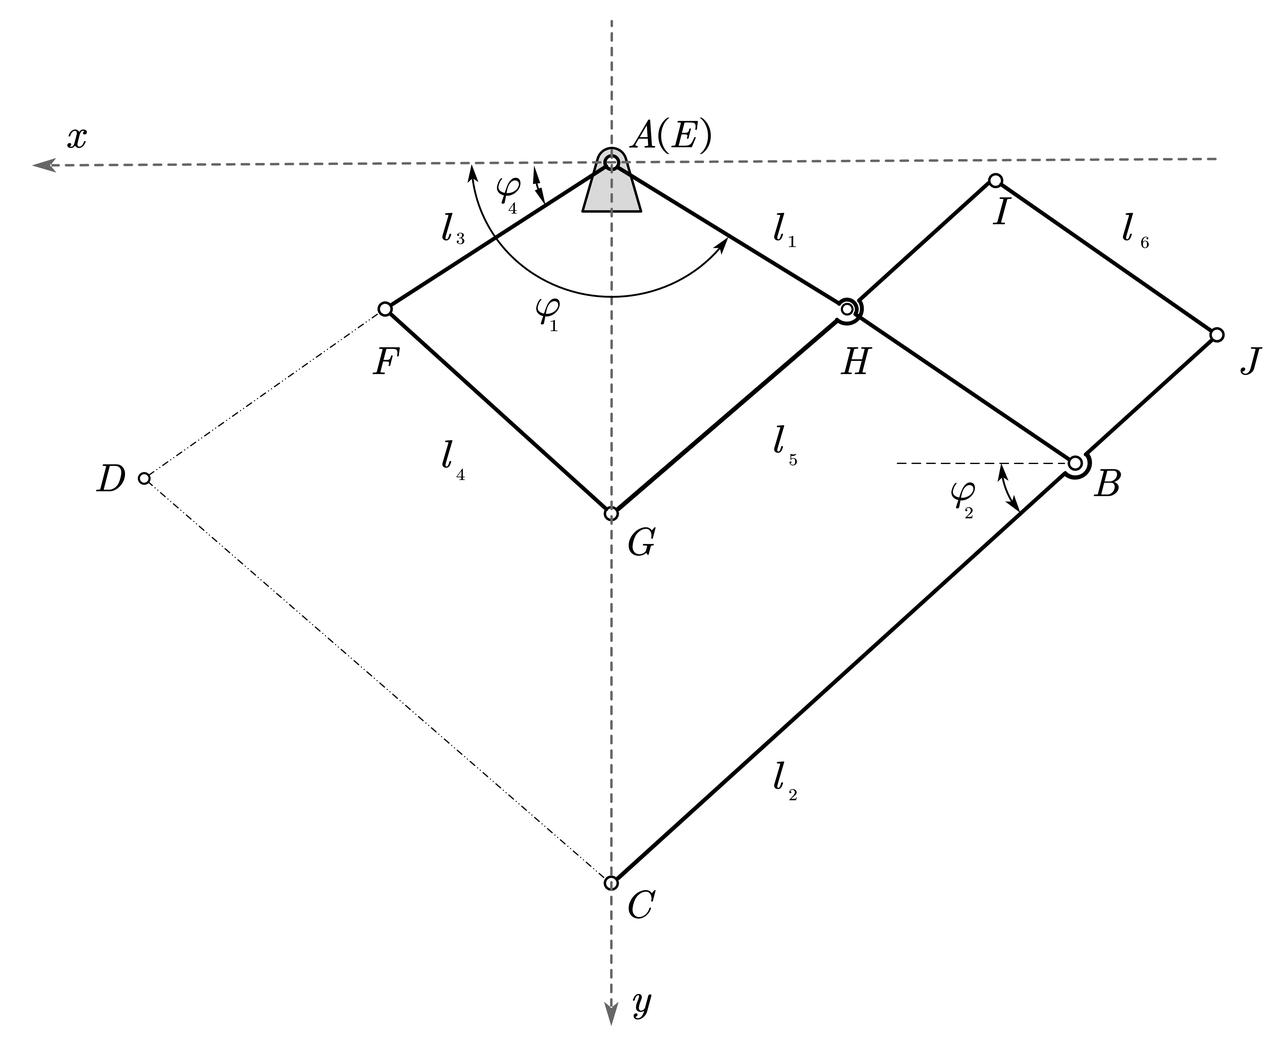
\includegraphics[width=0.72\textwidth]{figures/ch02/image1.png}
  \caption{腿部连杆机构简图}
\end{figure}

根据整机尺寸限制与越障指标要求，腿部连杆尺寸的设计直接决定了机器人的运动范围。本设计中的六杆机构关键参数如下：

\begin{itemize}
  \item 驱动曲柄长度（$l_3$）：取 $AF = AH = 86.4\,\mathrm{mm}$。此长度决定了腿部摆动的幅度，较短的曲柄有利于减小电机负载力臂。
  \item 从动连杆长度（$l_2$）：取 $CJ = 250.16\,\mathrm{mm}$。较长的从动杆能够保证足端具有足够的伸展范围，以满足 $20\,\mathrm{cm}$ 的跳跃缓冲行程。
\end{itemize}

基于上述尺寸，对单腿的垂直活动范围进行计算：

\begin{equation}
  H_{\max} = AB + BC = 160 + 196 = 356\,\mathrm{mm}
\end{equation}

其中，$H_{\max}$ 表示最大伸展长度；当曲柄与连杆共线且垂直向下时，腿部达到最长。

\begin{equation}
  H_{\min} \approx 100\,\mathrm{mm}
\end{equation}

其中，$H_{\min}$ 表示最小收缩长度。受限于机械限位与传动角限制，设定曲柄向上旋转的极限夹角为水平以上 $30^\circ$，此时腿部收缩至最短。

\begin{equation}
  S_{\mathrm{eff}} = H_{\max} - H_{\min} \approx 256\,\mathrm{mm}
\end{equation}

该行程完全覆盖了设计指标中要求的越障高度，并为跳跃落地提供了充足的缓冲减速距离。

在 Python 中对该连杆参数的工作空间进行仿真：

\begin{figure}[H]
  \centering
  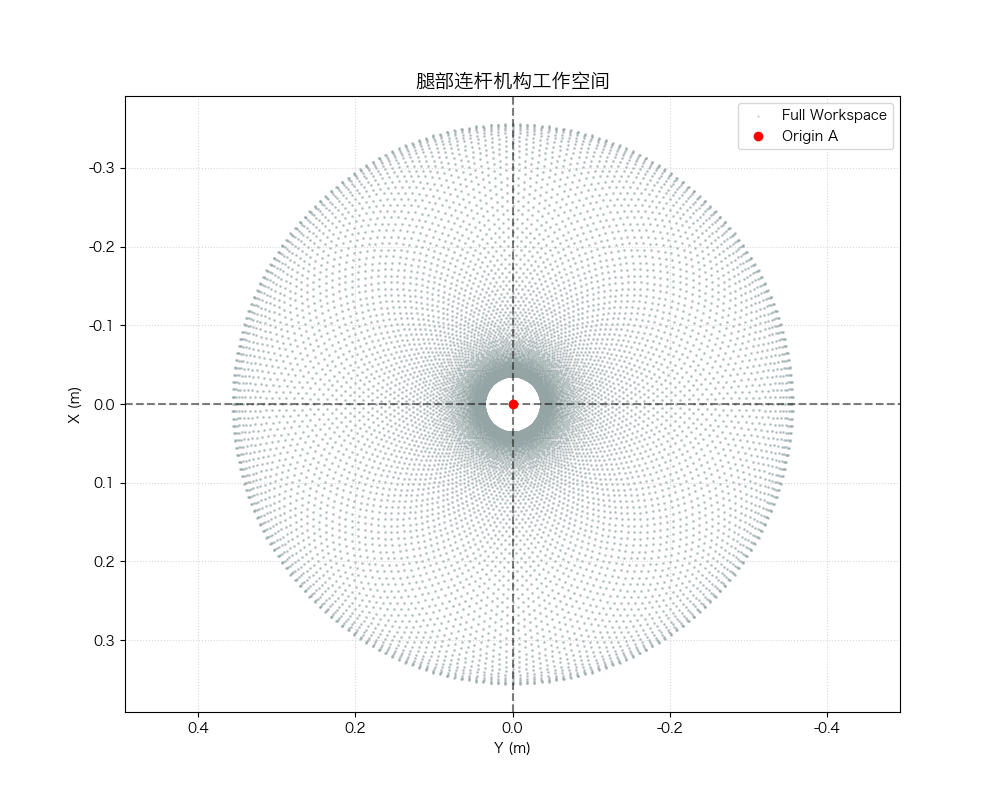
\includegraphics[width=0.72\textwidth]{figures/ch02/image2.png}
  \caption{腿部连杆工作空间示意图}
\end{figure}

由上图可知，该连杆参数下，腿部工作空间充裕，能够完成既定任务与指标。总结连杆参数至\tabref{tab:link-lengths}。

\begin{table}[htbp]
  \centering
  \caption{连杆参数汇总}\label{tab:link-lengths}
  \renewcommand{\arraystretch}{1.2}
  \begin{tabular}{cc}
    \toprule
    连杆代号 & 长度/m \\
    \midrule
    AF & 0.08640 \\
    FG & 0.10584 \\
    GI & 0.16000 \\
    IJ & 0.07360 \\
    JC & 0.25016 \\
    AB & 0.16000 \\
    \bottomrule
  \end{tabular}
\end{table}

下文分别从 6 个杆件开始，进行逐个设计。

\begin{figure}[H]
  \centering
  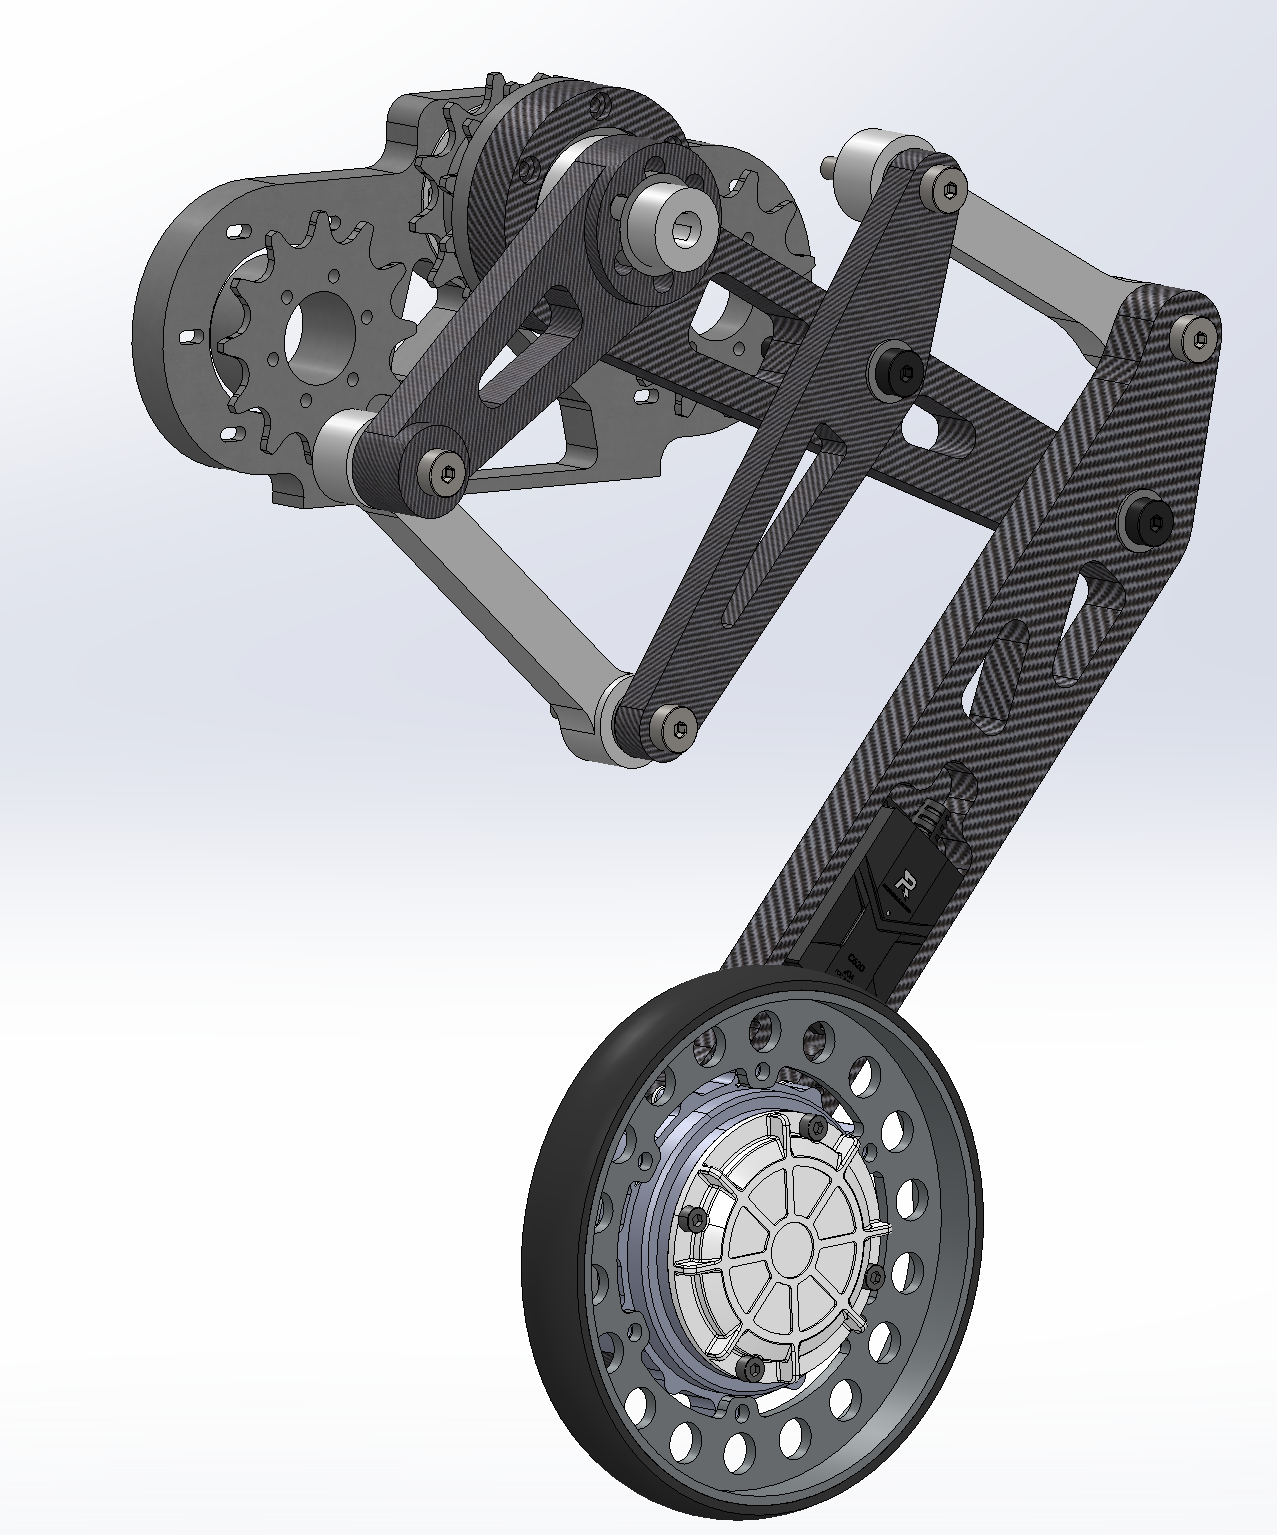
\includegraphics[width=0.6\textwidth]{figures/ch02/image3.png}
\end{figure}

\subsubsection*{B. 躯干设计}

躯干是机器人的主体，承载所有核心电子元件和电池，同时需要承载腿部髋关节。功能定位上作为控制中心、能源中心和力矩分配中心。

拟采用框架式结构的设计原则，最大化内部空间利用率，并合理布置重心。为了提高机器人的平衡性能，将电池等重物尽量靠近机器人的几何中心和地面，实现低重心设计。同时为了最大程度地简化结构复杂度，减轻整机重量，将腿部传动使用的髋关节也作为机器人躯干的一部分，两个髋关节之间使用镂空的板材进行连接，同时在躯干上方螺栓连接一个 3D 打印件作为电池架，最终形成一个部分封闭的箱式结构。

\begin{figure}[H]
  \centering
  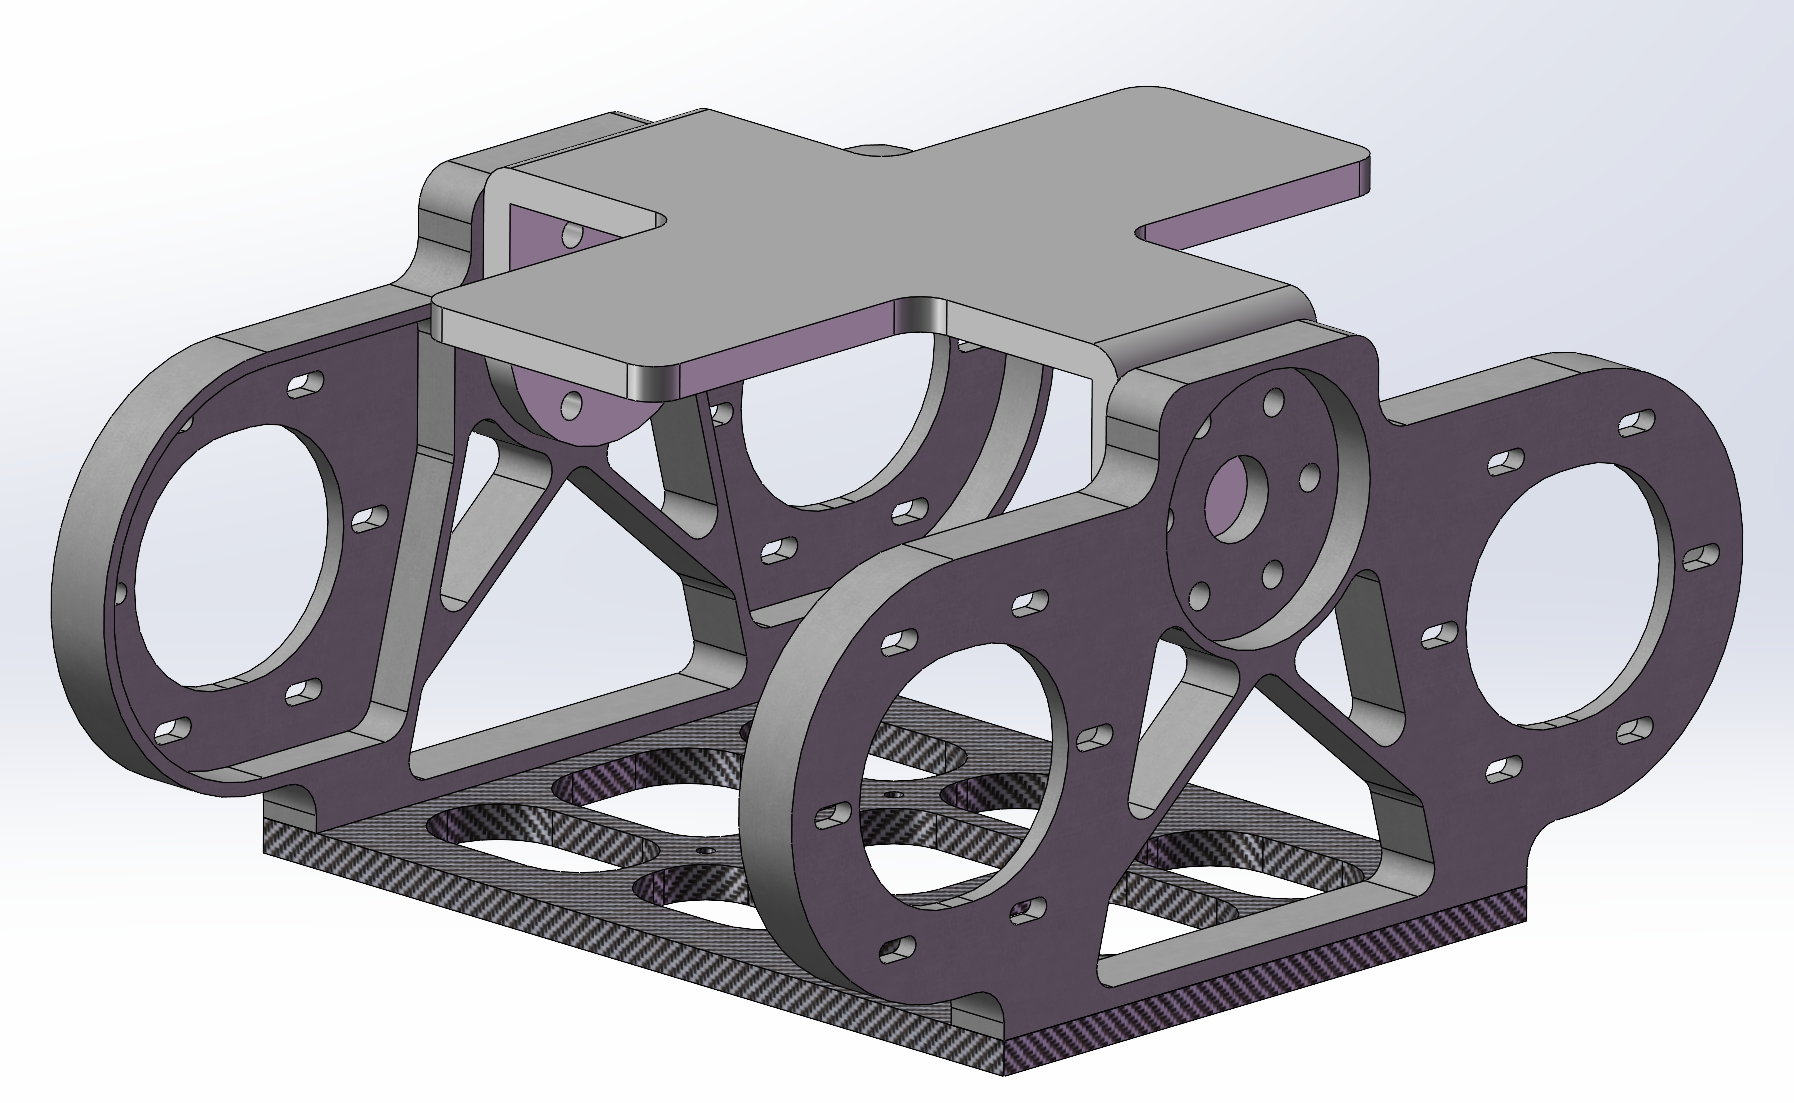
\includegraphics[width=0.6\textwidth]{figures/ch02/image4.png}
\end{figure}

优先采用碳纤维板材或高强度铝合金（如 7075/6061）进行加工，在保证结构刚度的前提下达到极致轻量化。

\subsubsection*{C. 关节与传动设计}

\paragraph{a. 髋关节轴系}
髋关节轴系采用嵌套式的二级轴系设计，运用两组轴承实现髋关节和膝关节自由度的传动。该结构不仅具备较高的承载能力与稳定性，还兼顾了运动灵活性与结构紧凑性，适用于人体下肢外骨骼、仿生机器人等对空间布局与传动效率要求较高的应用场景。

具体而言，髋关节轴系由内、外两层轴系组成。内轴系主要负责膝关节的屈伸运动，外轴系则控制髋关节的屈伸与旋转。两组轴承分别布置于轴系的关键支撑位置，有效分散运动过程中的径向与轴向载荷，降低摩擦损耗，提升传动效率与使用寿命。

\begin{figure}[H]
  \centering
  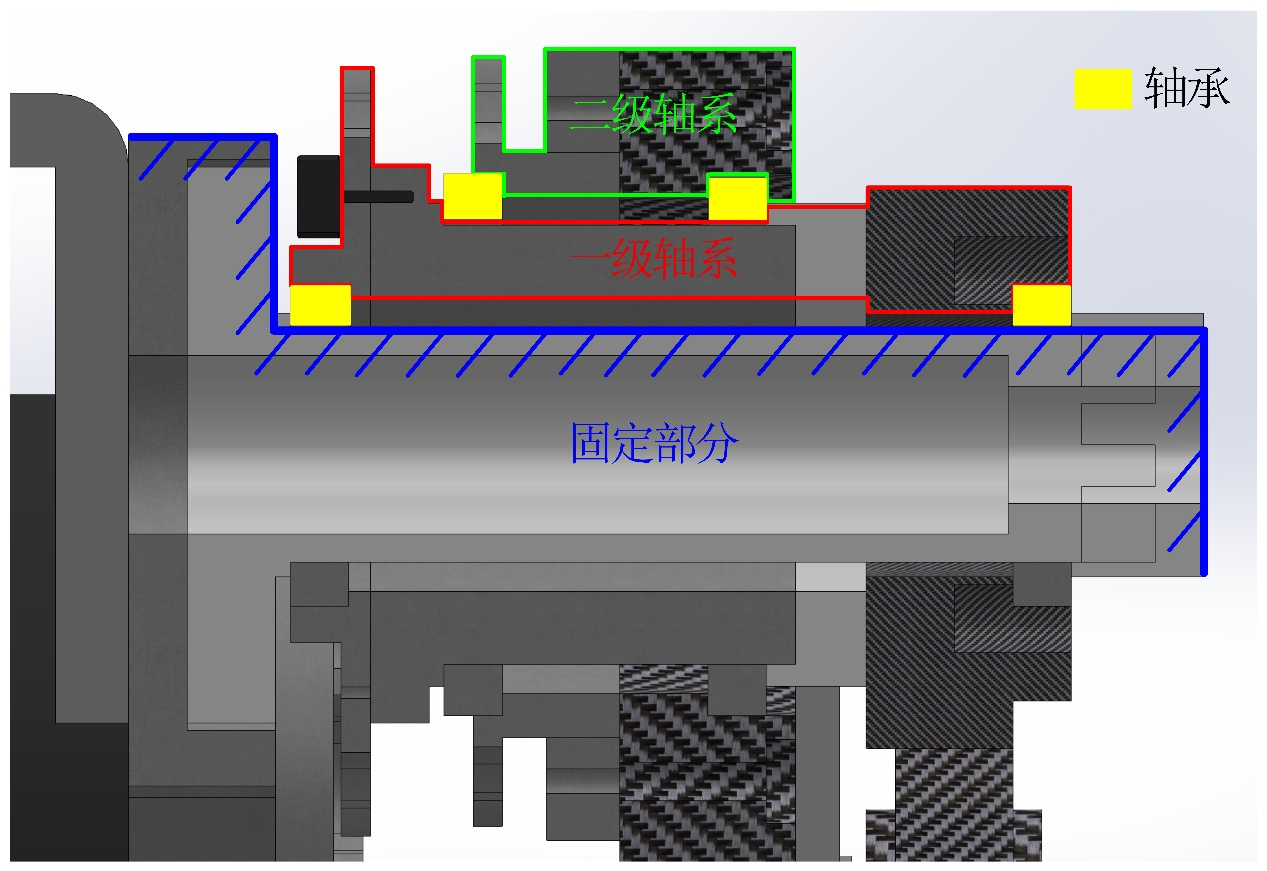
\includegraphics[width=0.48\textwidth]{figures/ch02/image5.jpeg}
\end{figure}

\paragraph{b. 链传动设计}
为了满足“驱动电机后置”及“轻量化”设计需求，本设计选用成熟度高、强度重量比优异的自行车链传动系统作为腿部力矩传递方案。

本系统选用 9 速自行车链条作为传动介质。相较于工业同步带或微型链条，该方案具有以下显著优势：

\begin{itemize}
  \item 极高的抗拉强度：9 速链条专为应对骑行中的瞬间高爆发力设计，其销轴抗拉载荷超过 $9000\,\mathrm{N}$，远超电机峰值负载需求。
  \item 轻量化与紧凑性：链条采用薄型高强度钢材制造，销轴长度约为 $6.6\,\mathrm{mm}$，能够显著减小腿部结构的横向厚度，符合整机紧凑设计的要求。
  \item 传动效率与耐受性：滚子链传动属于啮合传动，无弹性滑动，能保证精确的平均传动比。同时，自行车链条对沙尘、油污等非结构化环境具有较强的耐受性。
\end{itemize}

基于 2.3.1 节中确定的电机参数，对最恶劣工况（跳跃落地瞬间，峰值扭矩）进行静强度校核。有效圆周力（链条拉力）计算如下：

\begin{equation}
  F_t = \frac{2 T_{\text{peak}}}{d} = \frac{2 \times 12.5}{0.04907} \approx 509.5\,\mathrm{N}
\end{equation}

查阅主流品牌（如 Shimano/KMC）9 速链条技术规格，其最小破坏载荷满足：

\begin{equation}
  F_u \geq 8500\,\mathrm{N}
\end{equation}

计算安全系数：

\begin{equation}
  S = \frac{F_u}{F_t} = \frac{8500}{509.5} \approx 16.68
\end{equation}

校核结论表明，该链传动系统具有极高的安全冗余。即使在考虑冲击载荷系数 $K_A \approx 1.5$ 的情况下，链条仍工作在极其安全的范围内，几乎不存在断裂风险。

\begin{figure}[H]
  \centering
  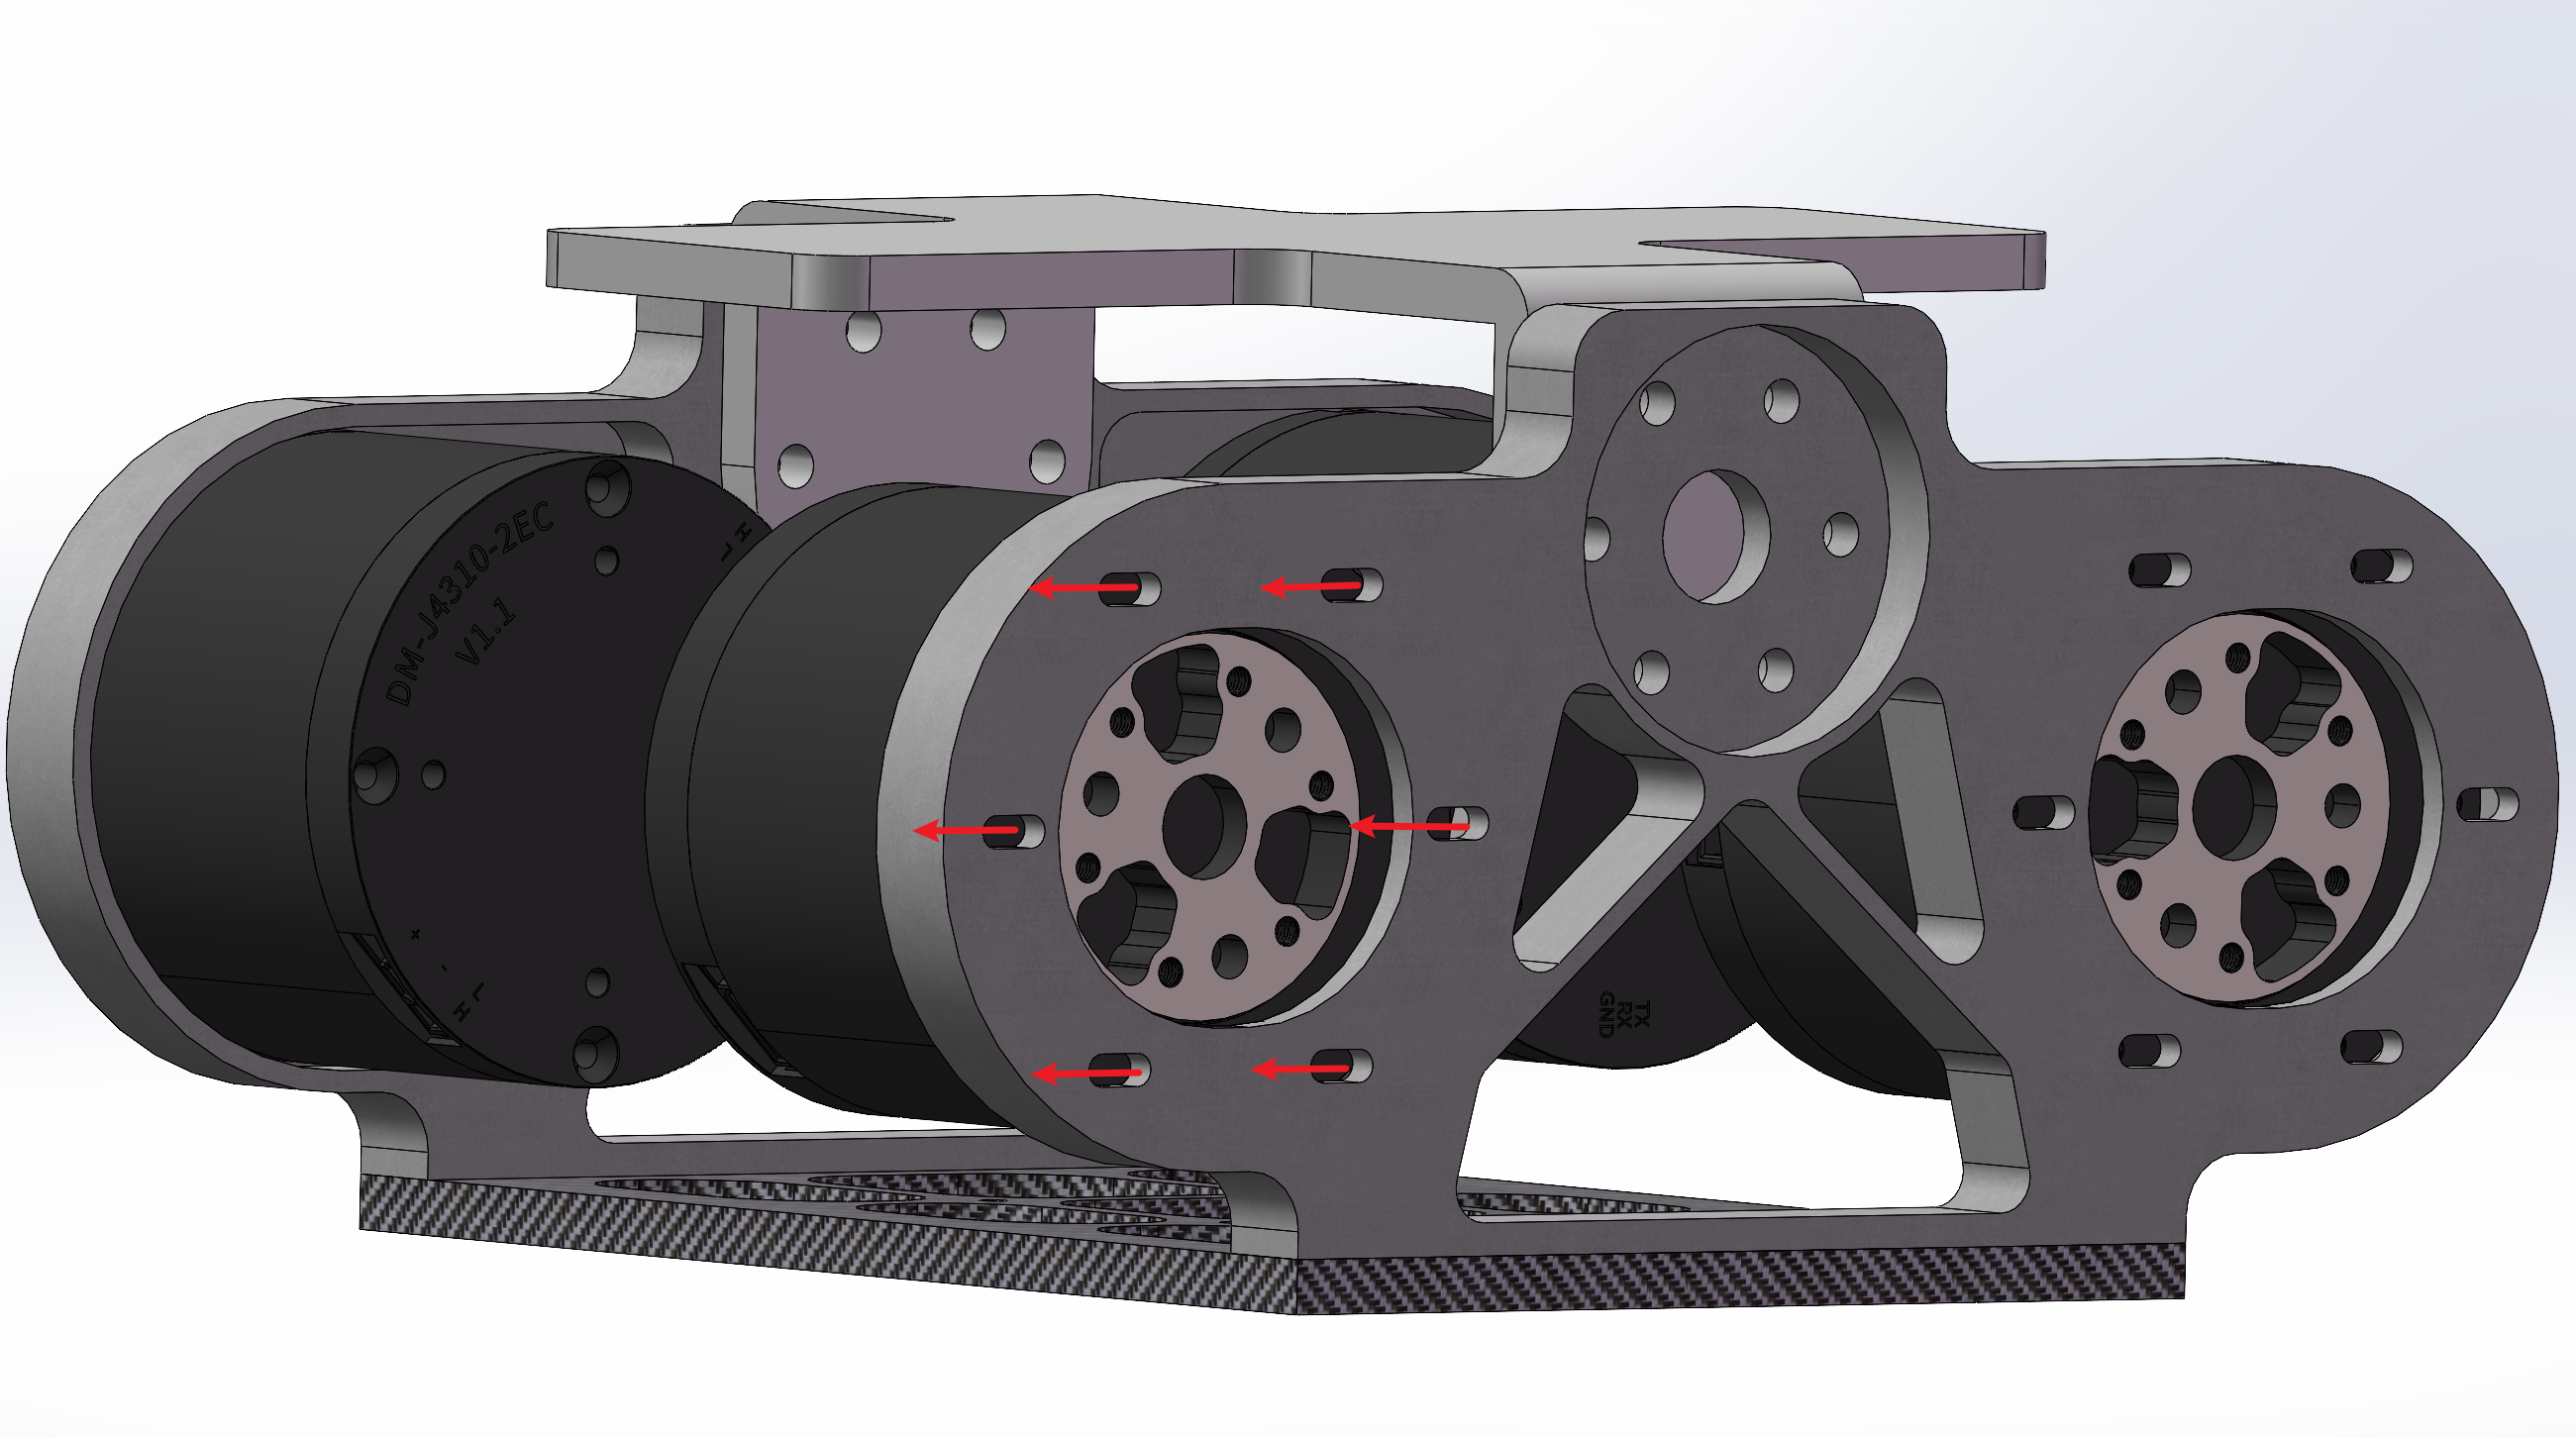
\includegraphics[width=0.6\textwidth]{figures/ch02/image6.png}
\end{figure}

链传动在长时间高频往复运动后，链条销轴与套筒之间会产生微量磨损，导致链条总长增加。若链条过松，会导致传动回差增大，影响机器人的倒立摆平衡控制精度，甚至在剧烈跳跃时发生脱链风险。

为了避免引入额外的弹簧张紧臂或惰轮机构增加簧上质量，本系统采用改变中心距的方式实现张紧。

\begin{itemize}
  \item 结构实现：在髋关节连接板（即电机安装座）上，驱动电机的安装孔位被设计为水平向滑槽。滑槽长度设计为 $7\,\mathrm{mm}$，允许电机定子沿水平方向进行 $\pm 4\,\mathrm{mm}$ 的位移调整。
  \item 调节原理：由于驱动链轮直接固定于电机输出轴，当松开电机固定螺栓并沿滑槽水平向外移动电机定子时，驱动链轮与从动链轮（连杆端）之间的几何中心距 $a$ 随之增大，从而拉紧链条。
  \item 优点：无需任何附加零件，仅通过机加工特征即可实现张紧功能，符合结构轻量化原则；相比于弹性张紧器，螺栓锁紧后的电机定子与机架形成刚性连接，保证了传动系统在高动态负载下的刚度，避免了弹性元件引入的系统谐振；当检测到链条松弛时，仅需微调电机位置并重新锁紧即可，便于日常维护与调试。
\end{itemize}

\subsection{驱动电机选型}

关节电机主要承担机器人的站立支撑、姿态调整以及跳跃腾空等任务。其中，最大跳跃起飞是峰值扭矩的极限工况，而“单腿半蹲支撑”是额定扭矩的典型工况。

\paragraph{1. 峰值扭矩需求（基于跳跃工况）}
假设机器人需要实现原地跳跃，腾空高度目标为 $H_{\text{jump}} = 0.3\,\mathrm{m}$（相对于起跳位置）。根据能量守恒定律，机器人离地瞬间的动能需转化为重力势能：

\begin{equation}
  \frac{1}{2} M v_{\text{takeoff}}^2 = M g H_{\text{jump}}
\end{equation}

解得起跳速度：

\begin{equation}
  v_{\text{takeoff}} = \sqrt{2 g H_{\text{jump}}} \approx 2.42\,\mathrm{m/s}
\end{equation}

假设加速起跳阶段的有效伸腿行程为 $h_{\text{acc}} = 0.15\,\mathrm{m}$，根据动能定理，地面对足端的平均反作用力需满足：

\begin{equation}
  \left(F_{\text{ground}} - Mg\right) h_{\text{acc}} = \frac{1}{2} M v_{\text{takeoff}}^2
\end{equation}

代入数据计算得：

\begin{equation}
  F_{\text{ground}} = \frac{M g H_{\text{jump}}}{h_{\text{acc}}} + Mg
  = \frac{5 \times 9.8 \times 0.3}{0.15} + 49 = 147\,\mathrm{N}
\end{equation}

根据虚功原理，足端力与关节力矩的关系由雅可比矩阵 $J$ 决定，即 $\tau = J^\mathsf{T} F$。在典型的半蹲姿态下（大腿与小腿夹角约为 $90^\circ$），力臂最长。设大腿与小腿连杆长度均为 $L_{\text{link}} \approx 0.15\,\mathrm{m}$，此时所需的峰值关节力矩估算为：

\begin{equation}
  T_{\text{peak}} \approx F_{\text{peak}} \cdot L_{\text{link}} \cdot \sin \theta_{\text{eff}}
\end{equation}

取有效力臂系数约为 0.7（考虑连杆角度），则：

\begin{equation}
  T_{\text{peak}} \approx 147 \times 0.15 \times 0.7 \approx 15.4\,\mathrm{N\cdot m}
\end{equation}

由于机器人采用双电机并联驱动（或髋膝耦合），实际单电机承担峰值力矩会有所降低。考虑到减速比增益，所选电机峰值扭矩需接近 $10 \sim 15\,\mathrm{N\cdot m}$ 范围。

\paragraph{2. 额定扭矩需求（基于站立工况）}
在机器人处于单腿支撑或静止半蹲维持姿态时，电机需提供持续力矩对抗重力。最恶劣工况为单腿支撑整机重量，且处于力臂最大的蹲姿：

\begin{equation}
  T_{\text{rated}} = Mg \cdot L_{\text{link}} \cdot \sin 45^\circ
  \approx 5 \times 9.8 \times 0.15 \times 0.707 \approx 5.2\,\mathrm{N\cdot m}
\end{equation}

考虑到通常为双腿支撑，单腿实际负载减半，即约为 $2.6\,\mathrm{N\cdot m}$。

选型结论：本设计选用的无刷减速电机，额定扭矩为 $3.5\,\mathrm{N\cdot m}$，峰值扭矩为 $12.5\,\mathrm{N\cdot m}$。其中，额定扭矩满足持续支撑需求，峰值扭矩接近极限跳跃估算值，配合双腿协同工作可满足爆发力需求。

\setcounter{subsection}{3}
\subsection{电机选型}

机器人的动态性能与复杂场景下的运动能力主要取决于执行器的性能。根据上文中的简单计算，本设计对关键执行器进行了如下选型：

关节驱动电机：选用额定扭矩为 $3.5\,\mathrm{N\cdot m}$、峰值扭矩为 $12.5\,\mathrm{N\cdot m}$ 的高性能无刷减速电机。$3.5\,\mathrm{N\cdot m}$ 的额定扭矩能够为髋关节和膝关节提供充足的持续驱动力，电机内置的行星减速机构可将峰值输出扭矩提升至更高水平，同时该电机具有 MIT 模式、速度模式、位置模式三种控制模式，能够满足机器人在跳跃落地瞬间的高冲击负载需求以及站立平衡时的力矩控制精度。

\begin{figure}[H]
  \centering
  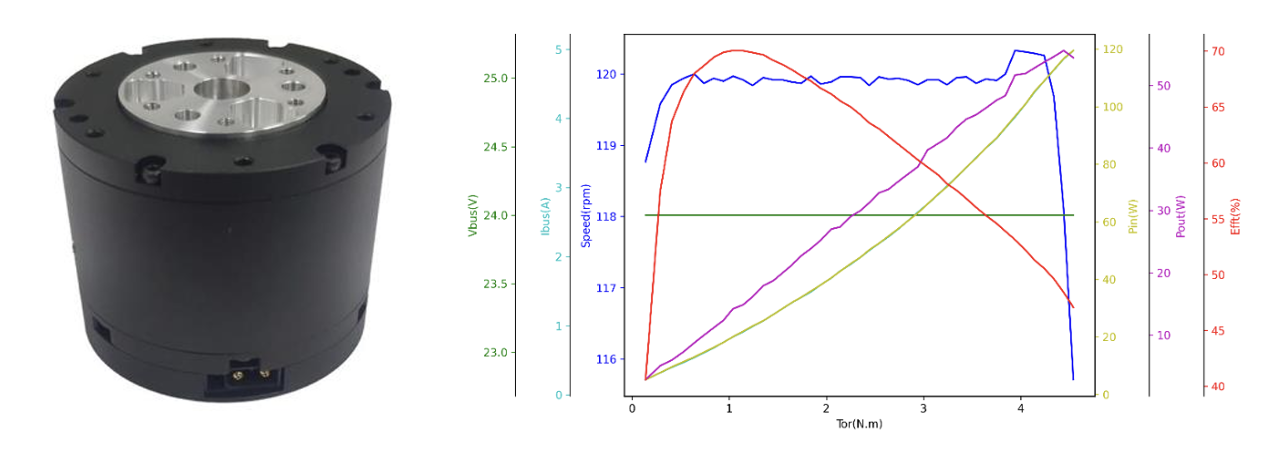
\includegraphics[width=0.4\textwidth]{figures/ch02/image7.png}
\end{figure}

轮毂电机：选用额定扭矩为 $2.5\,\mathrm{N\cdot m}$ 的减速轮毂电机。该轮毂电机直接集成于足底，省去了复杂的传动链，极大地降低了足部惯量。$2.5\,\mathrm{N\cdot m}$ 的额定扭矩对于 $5\,\mathrm{kg}$ 级的机器人而言，能够提供充沛的地面驱动力，确保在轮式模式下具备优秀的加速性能和爬坡能力。

\begin{figure}[H]
  \centering
  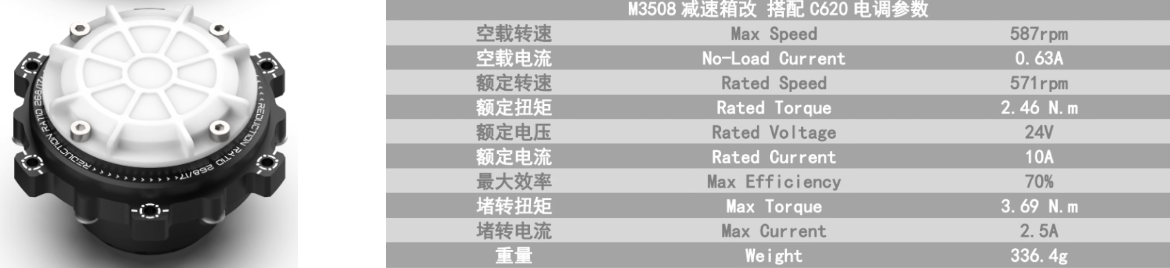
\includegraphics[width=0.4\textwidth]{figures/ch02/image8.png}
\end{figure}

\section{移动系统设计}

本混合式双轮足机器人以混合式结构作为方向，通过在串联主链中引入局部并联支链，旨在兼顾运动灵活性与结构刚性。机器人主要由核心躯干、两套对称的腿部模块以及两个驱动轮构成。

\subsection{轮组机械结构设计}

本机器人的驱动轮并非独立于腿部，而是集成在足部关节处。驱动轮固定于腿部最末端的踝关节之下，作为机器人在轮式模式下的主要支撑点和执行器。

\begin{figure}[H]
  \centering
  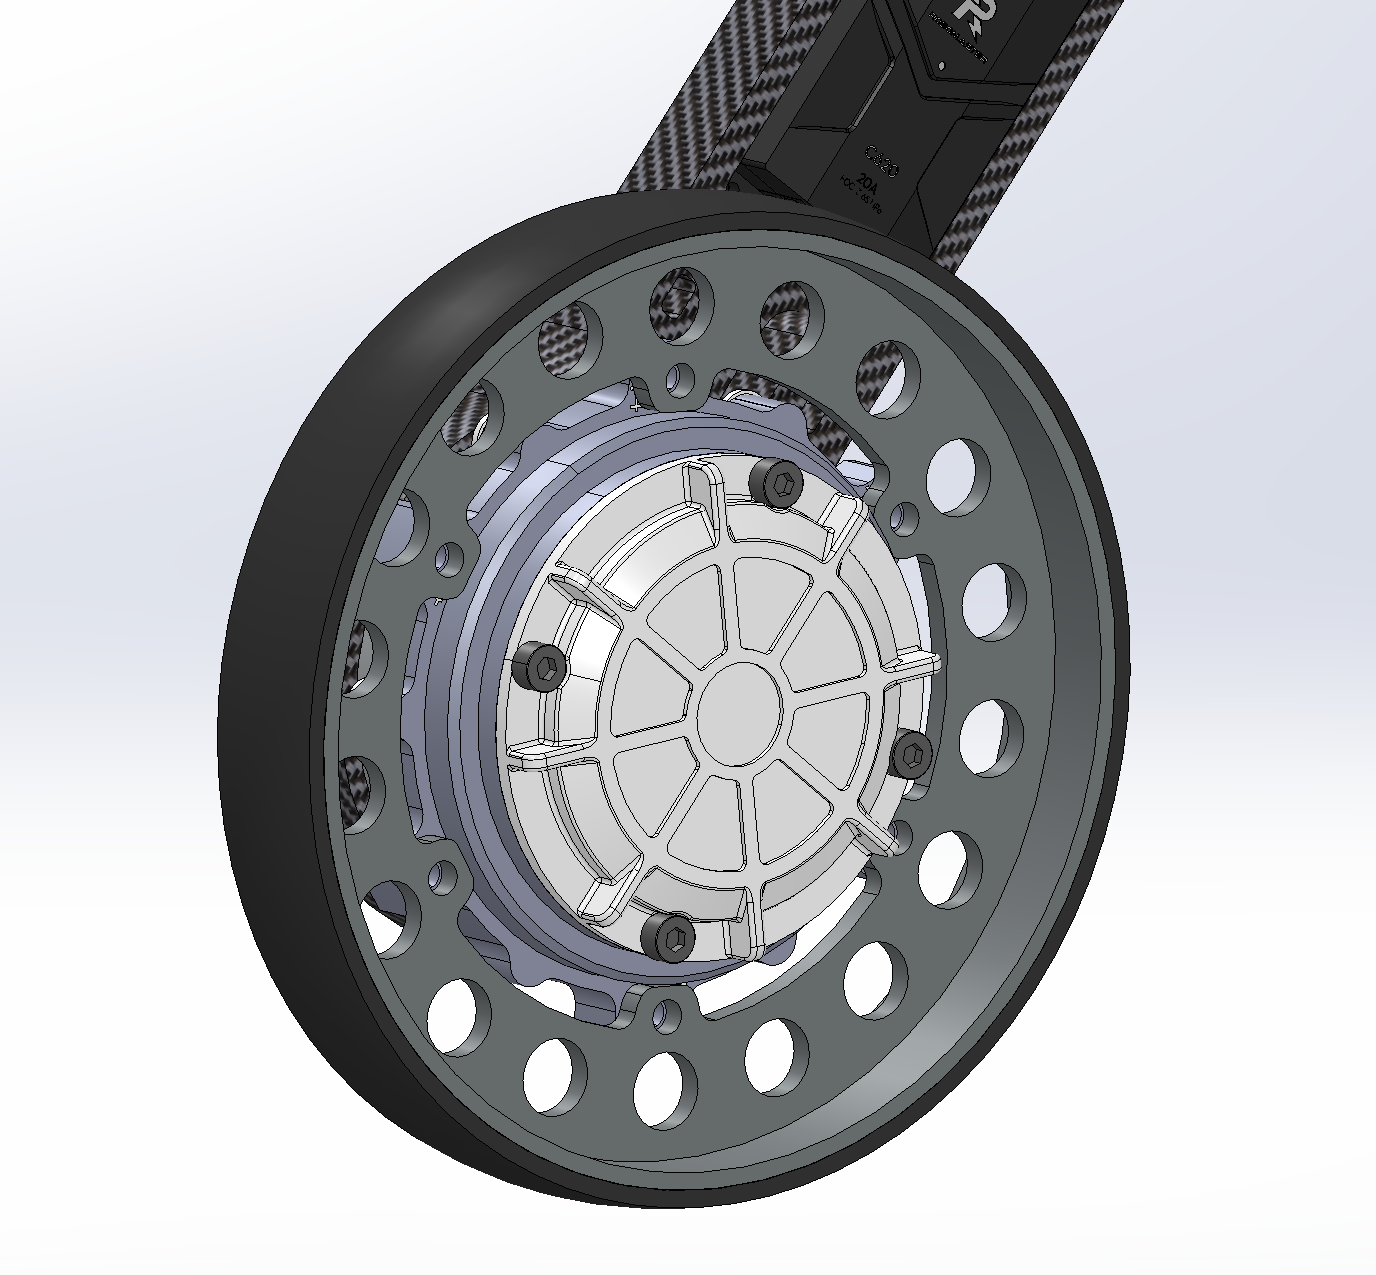
\includegraphics[width=0.38\textwidth]{figures/ch02/image9.png}
\end{figure}

这种设计最大限度地减少了额外的驱动机构和结构件，是实现轻量化的关键。

\subsection{电机选型}

轮毂电机主要决定机器人的移动速度、加速度及爬坡能力。

\subsubsection*{A. 加速度与最大速度需求}

设计指标要求最大移动速度 $v_{\max} \geq 2\,\mathrm{m/s}$。设轮子半径 $r = 0.06\,\mathrm{m}$。

电机转速需求：

\begin{equation}
  \omega = \frac{v_{\max}}{r}
  = \frac{2}{0.06}
  \approx 33.3\,\mathrm{rad/s}
  \approx 318\,\mathrm{RPM}
\end{equation}

所选轮毂电机额定转速通常在此范围内。考虑加速性能，假设机器人在 $t = 0.5\,\mathrm{s}$ 内从静止加速至 $2\,\mathrm{m/s}$，所需加速度为

\begin{equation}
  a = 4\,\mathrm{m/s^2}
\end{equation}

所需驱动力为

\begin{equation}
  F_{\text{drive}} = Ma = 5 \times 4 = 20\,\mathrm{N}
\end{equation}

考虑滚动摩擦阻力（设系数 $\mu = 0.05$），总牵引力为：

\begin{equation}
  F_{\text{total}} = Ma + \mu Mg
  = 20 + 0.05 \times 5 \times 9.8
  = 22.45\,\mathrm{N}
\end{equation}

对应总扭矩需求：

\begin{equation}
  T_{\text{acc}} = F_{\text{total}} \cdot r
  = 22.45 \times 0.06
  \approx 1.35\,\mathrm{N\cdot m}
\end{equation}

\subsubsection*{B. 爬坡能力需求}

假设机器人需攀爬 $\alpha = 20^\circ$ 的斜坡。重力沿斜坡分量为：

\begin{equation}
  F_{\text{climb}} = Mg \sin \alpha
  = 5 \times 9.8 \times 0.342
  \approx 16.8\,\mathrm{N}
\end{equation}

对应爬坡扭矩：

\begin{equation}
  T_{\text{climb}} = F_{\text{climb}} \cdot r
  = 16.8 \times 0.06
  \approx 1.01\,\mathrm{N\cdot m}
\end{equation}

\subsubsection*{C. 选型结论}

双轮驱动下，单轮所需最大扭矩约为 $0.7 \sim 1.0\,\mathrm{N\cdot m}$。

\section{整机}
